\documentclass[11pt, a4paper]{article}

\usepackage[utf8]{inputenc}
\usepackage{listings}             % Include the listings-package for c++,java,idl
\usepackage[margin=0.75in]{geometry}
\usepackage{graphicx}
\usepackage{url}
% \usepackage[ngerman]{babel}

\title{JMS-Chat}
\author{Elias Frantar, Gary Ye (4BHIT)}
\date{\today{}, Wien}
\begin{document}

% Pretty Code formatting
\lstset{basicstyle=\ttfamily\small,
        keywordstyle=,
        commentstyle=\itshape,
        numbers=left,                   % where to put the line-numbers
        stepnumber=1,					% line number incrementing
        breaklines=true,					% line wrapping on
        numberstyle=\tiny,				% line number style	
        showstringspaces=false,			
        abovecaptionskip=0pt,
        belowcaptionskip=0pt,
        xleftmargin=\parindent,
        fontadjust}

\maketitle
\newpage
\tableofcontents
\newpage

\section{Aufgabenstellung}
Implementieren Sie eine Chatapplikation mit Hilfe des Java Message Service. Verwenden Sie Apache ActiveMQ (http://activemq.apache.org) als Message Broker Ihrer Applikation. Das Programm soll folgende Funktionen beinhalten:

Benutzer meldet sich mit einem Benutzernamen und dem Namen des Chatrooms an. 
Beispiel für einen Aufruf: 

\begin{lstlisting}
vsdbchat <ip_message_broker> <benutzername> <chatroom>
\end{lstlisting}

Der Benutzer kann in dem Chatroom (JMS Topic) Nachrichten an alle Teilnehmer eine Nachricht senden und empfangen. 
Die Nachricht erscheint in folgendem Format:
\begin{lstlisting}
<benutzername> [<ip_des_benutzers>]: <Nachricht>
\end{lstlisting}

Zusätzlich zu dem Chatroom kann jedem Benutzer eine Nachricht in einem persönlichen Postfach (JMS Queue) hinterlassen werden. Der Name des Postfachs ist die IP Adresse des Benutzers (Eindeutigkeit).

Nachricht an das Postfach senden: 
\begin{lstlisting}
MAIL <ip_des_benutzers> <nachricht>
\end{lstlisting}

Eignes Postfach abfragen: 
\begin{lstlisting}
MAILBOX
\end{lstlisting}

Der Chatraum wird mit den Schlüsselwort EXIT verlassen. Der Benutzer verlaesst den Chatraum, die anderen Teilnehmer sind davon nicht betroffen.
Gruppenarbeit: Die Arbeit ist in einer 2er-Gruppe zu lösen und über das Netzwerk zu testen! Abnahmen, die nur auf localhost basieren sind unzulässig und werden mit 6 Minuspunkten benotet!

\subsection{Quellen}
\begin{itemize}
\item http://activemq.apache.org/index.html
\item http://www.academictutorials.com/jms/jms-introduction.asp
\item http://docs.oracle.com/javaee/1.4/tutorial/doc/JMS.html\#wp84181
\item http://www.openlogic.com/wazi/bid/188010/How-to-Get-Started-with-ActiveMQ
\item http://jmsexample.zcage.com/index2.html
\item http://www.onjava.com/pub/a/onjava/excerpt/jms\_ch2/index.html
\item http://www.oracle.com/technetwork/systems/middleware/jms-basics-jsp-135286.html
\item http://java.sun.com/developer/technicalArticles/Ecommerce/jms
\end{itemize}

\newpage

\section{Aufwandsschätzung}
Installation Message Broker Apache ActiveMQ wurde im Unterricht durchgeführt und entfällt daher.

\begin{description}
\item[Alle Teammitglieder] \hfill \\
  \begin{tabular} {| l | l |}
    \hline
    Task & Tatsächlich \\ \hline
    Bekanntmachung mit JMS & 1.5h \\ \hline
    Planung & 1.5h \\ \hline
    \hline
    Gesamt & 3h \\ \hline
  \end{tabular}

\item[Frantar] \hfill \\

  \begin{tabular} {| l | l | l |}
    \hline
    Task & Schätzung & Tatsächlich \\ \hline
    Implementierung JMSChat & 1.5h & 0.75h \\ \hline
    Implementierung JMSMail & 1.5h & 1.5h \\ \hline
    Protokoll & 4h & 4h \\ \hline
    \hline
    Gesamt & 7h & 6.75h \\ \hline
  \end{tabular}

\item[Ye] \hfill \\
    \begin{tabular} {| l | l | l |}
      \hline
      Task & Schätzung & Aufwand \\ \hline
      SyntaxChecker Implementierung & 0.75h & 0.25h \\ \hline
      SyntaxChecker Test & 0.5h & 0.5h \\ \hline
      JMS-User Implementierung & 2h & 0.5h \\ \hline
      Protokoll & 5h & 4h \\ \hline
      \hline
      Gesamt & 8.25h & 5.25h \\ \hline
    \end{tabular}
\end{description}

\section{Installation}
Herunterladen der Installationsdateien von \cite{activemqdownload} mit Hilfe von wget.
\begin{lstlisting}
 wget http://www.eu.apache.org/dist/activemq/apache-activemq/5.7.0/apache-activemq-5.7.0-bin.tar.gz
\end{lstlisting}
Entpacken der Installationsdateien mit
\begin{lstlisting}
 tar xf apache-activemq-5.7.0-bin.tar.gz
\end{lstlisting}
Falls benötigt - ändern der Ausführungsrechte von bin/activemq mit chmod u+x, damit die Datei ausführbar wird.
Danach das Binary File starten mit
\begin{lstlisting}
bin/activemq start
\end{lstlisting}

Man kann mithilfe von ``bin/activemq status'' überprüfen, ob activemq korrekt gestartet wurde.

\newpage

\section{Neue Technologien}
\subsection{Grundlagen}
Das Java Message Service (JMS) \cite{activemqtut1} ist eine auf Java basierende Message Oriented Middleware (MOM) zum Versenden von Nachrichten zwischen 2 oder mehr Systemen.
Grundlegend funtkioniert dies folgendermaßen:
Auf der MOM (meist auf einem Server liegend) können Topics und Queues angelegt werden.
In diese können JMS-Teilnehmer Nachrichten versenden bzw. Nachrichten von ihnen empfangen/auslesen. (sofern entsprechende Zugriffsrechte vorhanden)
D.h. alle Systeme kommunizieren nur über Nachrichten (Objekte) welche über die MOM ausgetauscht werden.

Genauere Informationen über die Implementierung sind in den folgenden zwei Abschnitten zu finden.

\subsection{JMS-Topic}
Ein JMS-Topic ist, ähnlich wie Chat-Room, ein auf der MOM liegender Ort in den Nachrichten gesendet werden können. Ein JMS-Teilnehmer kann ein Topic
subscriben und erhält dadurch alle Nachrichten, die an das Topic gesendet werden (auch die eigenen).

Im folgenden Abschnitt ist die Implementierung der Verwendung eines JMS-Topics mithilfe von Code-Snippets erläutert.

\begin{lstlisting}[language=Java]
ConnectionFactory connectionFactory = new ActiveMQConnectionFactory(url);
connection = connectionFactory.createConnection();
connection.start();
\end{lstlisting}

Als erstes muss eine Verbindung mit dem JMS hergestellt werden. Dazu wird mithilfe der ActiveMQConnectionFactory eine Connection mit der JMS-Server-URL
hergestellt.

\begin{lstlisting}[language=Java]
session = connection.createSession(false, Session.AUTO_ACKNOWLEDGE)
\end{lstlisting}

Als nächstes kann mithilfe der erfolgreichen Verbindung eine JMS-Session erstellt werden. Durch dieses Session können im Anschluss Sender, Empfänger, sowie
Topics oder Queues erstellt werden.

\begin{lstlisting}[language=Java]
destination = session.createTopic(subject);

producer = session.createProducer(destination);
producer.setDeliveryMode(DeliveryMode.NON_PERSISTENT);
		
consumer = session.createConsumer(destination);
\end{lstlisting}

Wie oben bereits erwähnt wird nun durch die Session ein Topic, sofern es nicht bereits existiert, erstellt.
Im Anschluss werden noch ein Nachrichtensender (producer), welcher Nachrichten versendet, die nur temporär auf dem Server gespeichert werden und ein Nachrichtenempfänger,
welcher ein Topic subscribt und dementsprechend allen in diesem Topic eintreffende Nachrichten empfängt, erstellt.

\begin{lstlisting}[language=Java]
TextMessage message = (TextMessage)consumer.receive();
System.out.println(message.getText());
message.acknowledge();
\end{lstlisting}

Nun kann durch den Consumer eine Nachricht empfagen werden. Diese Methode blockiert solange bis sie eine Nachricht erhält. Aus dieser Nachricht kann im
Anschluss nun zum Beispiel der Textinhalt ausgelesen werden. Um dem Server zu bestätigen, dass diese Nachricht erhalten wurde und sie nicht nochmals gesendet
werden muss, wird abschließend noch acknowledge() aufgerufen.

\begin{lstlisting}[language=Java]
TextMessage message_to_send = session.createTextMessage(username + " " +  ip + ": " + message);
producer.send(message_to_send);
\end{lstlisting}

Mit dem Producer können Nachrichten an das festgelegte Topic verschickt werden. Dazu wird zuerst ein MessageObject (z.B. TextMessage) erzeugt, welches
anschließend durch send() versendet werden kann.

\subsection{JMS-Queue}
Eine Queue ist, ähnlich wie ein Topic, ein auf der MOM liegender Ort. Der Unterschied ist nur das in eine Queue zwar ebenfalls Nachrichten gesendet werden
können. Diese aber manuell ausgelesen werden müssen. Das Auslesen geschieht außerdem nach dem Queue-Prinzip, also First in First out. Zusätzlich bleiben
Nachrichten in der Queue gespeichert, sofern sie nicht explizit gelöscht werden.

Im folgenden Abschnitt ist die Implementierung der Verwendung einer JMS-Queue mithilfe von Code-Snippets erläutert.

\begin{lstlisting}[language=Java]
ConnectionFactory connectionFactory = new ActiveMQConnectionFactory(url);
connection = connectionFactory.createConnection();
connection.start();
			
session = connection.createSession(false, Session.AUTO_ACKNOWLEDGE);
\end{lstlisting}

Die Connection, sowie die Session, werden äquivalent zur in JMS-Topic beschriebenen Lösung umgesetzt.

\begin{lstlisting}[language=Java]
queue = session.createQueue(mailbox);
\end{lstlisting}

Aus einer Session kann, sowie ein Topic, eine Queue erstellt werden. Auch diese wird nur erzeugt sollte diese nicht bereits schon existieren.

\begin{lstlisting}[language=Java]
browser = session.createBrowser(queue);

producer = session.createProducer(queue);
producer.setDeliveryMode(DeliveryMode.NON_PERSISTENT);
\end{lstlisting}

Durch eine Session kann mit Übergabe einer Zielqueue QueueBrowser erstellt werden. Durch diesen kann der Inhalt einer Queue ausgelesen werden.
Äquivalent funktioniert das Erstellen eines Producers, also einer JMS-Komponente, die es ermöglicht Nachrichten an eine Queue zu senden.

\begin{lstlisting}[language=Java]
TextMessage msg = session.createTextMessage(message);
producer.send(msg);
\end{lstlisting}

Durch einen Producer können, genauso wie an ein Topic, Nachrichten versendet werden.

\begin{lstlisting}[language=Java]
Enumeration<?> messages = browser.getEnumeration();
while(messages.hasMoreElements()) {
	TextMessage message = (TextMessage)messages.nextElement();
	if(message.getText() != null) {
		mails.add(message.getText()); // save text of mail
		message.acknowledge();
	}
}
\end{lstlisting}

Mit einem Browser kann eine Liste aller sich in der Queue befindenden Nachrichten augelesen werden. Diese können nun in Sendungsreihenfolge nacheinander
ausgelesen werden.

\newpage

\section{Aufgetretene Probleme}

\subsection{Installation}

Für das Debian-Image muss eine Änderung durchgeführt werden, damit Apache Active MQ gestartet werden kann.
Öffnen Sie die Datei bin/activemq mit einem Editor Ihrer Wahl 
Suchen Sie nach folgender Zeile
%       ACTIVEMQ_OPTS_MEMORY="-Xms1G -Xmx1G"
Ersetzen Sie diese Zeile mit:
%       ACTIVEMQ_OPTS_MEMORY="-Xms512M -Xmx512M"
\subsection{IP Addresse}
Man kann mittels ActiveMQ nicht direkt die IP Addressen von dem Sender herausfinden. Siehe 
%TODO
Deshalbe wurde beschlossen, dass der User sie selber angibt, indem er das Programm das zu verwendende Interface übergibt. Von dem Interface wird die IP-Adresse ermittelt und anschließend zum Austauschen von Nachrichten übernommen.

\newpage

\section{Testing}

\subsection{Systemtest}
Sämtliche Systemtests wurden über das Netzwerk durchgeführt.
Als Testumgebung wird eine ActiveMQ auf einem in einer virtuellen Maschine laufenden Debian-Server eingesetzt. 3 Hosts (1 Debian + 2 Windows) verbinden sich
mit diesem Server. Die Hostmaschinen und der Server sind nur über das Netzwerk verbunden.

In den folgenden Abschnitten sind die einzelnen Testcases mit Ergebnissen detailliert dokumentiert.

\subsubsection{Chat}
Zum Testen des Chats verbinden sich 3 Clients im Chatroom 'Kryptos' mit dem JMS-Server.
Anschließend werden Nachrichten von allen 3 Seiten ausgetauscht.

Erwartet: Alle Nachrichten kommen mit Sendernamen auf allen 3 Hosts an.

\begin{center}
  \begin{description}
    \item[user1] \hfill \\ 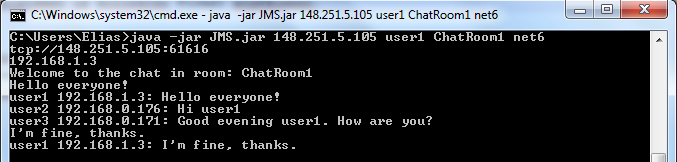
\includegraphics[width=5in]{pic/chat_user1.png}
    \item[user2] \hfill \\ 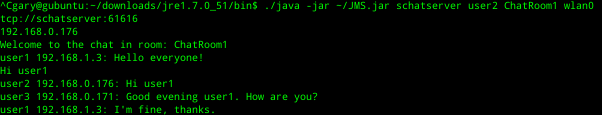
\includegraphics[width=5in]{pic/chat_user2.png}
    \item[user3] \hfill  \\ 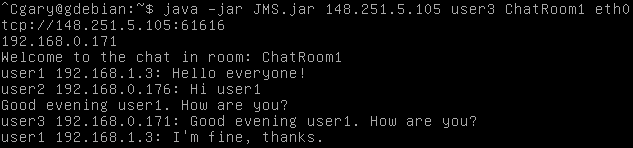
\includegraphics[width=5in]{pic/chat_user3.png}
  \end{description}
\end{center}

Ergebnis: Wie erwartet, sind alle Nachrichten auf allen 3 verschiedenen Hostsystemen im korrekten Format angekommen.

\subsubsection{Mail}
Zum Testen des Mailservices verbinden sich erneut 3 Clients im Chatroom 'Kryptos' mit dem ActiveMQ-Server.
Nun senden verschiedene Clients verschiedene Nachrichten an den 1. auf Windows befindenden Host.
Dieser ruft dann seine Mailbox ab und liest damit alle empfangenen Nachrichten aus.

Ablauf:
\begin{itemize}
	\item user1, user2 und user3 verbinden sich erneut mit 'ChatRoom1'
	\item user2: MAIL 'user1IP' Dear user1, I'm just testing the brandnew JMS Mailservice ;)
	\item user2: Hey user1, check out your mails!
	\item user1: MAILBOX
	\item user1: Received it!
	\item user3: MAIL 'user1IP' a test mail from me ;)
	\item user1: MAILBOX
	\item user1: It works!
\end{itemize}

Erwartet: Alle Nachrichten landen in der Mailbox des Empfängers. Bei Aufruf von MAILBOX werden diese in korrekter Reihenfolge ausgelesen.

\begin{center}
\begin{description}
\item[user1] \hfill \\   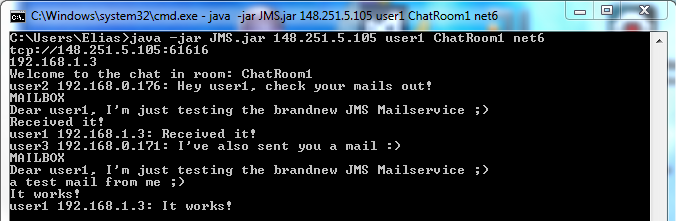
\includegraphics[width=6in]{pic/mail_user1.png}
\item[user2] \hfill \\   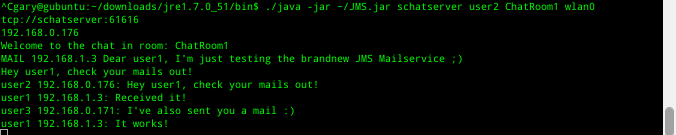
\includegraphics[width=6in]{pic/mail_user2.png}
\item[user3] \hfill \\   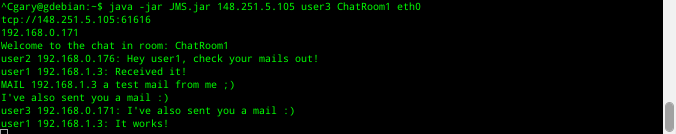
\includegraphics[width=6in]{pic/mail_user3.png}
\end{description}
\end{center}

Erwartet: Alle Nachrichten befinden sich in der Mailbox des Empfängers.

Ergebnis: Wie erwartet scheinen alle Nachrichten in der Mailbox des Empfängers auf. Zusätzlich werden diese dauerhaft gespeichert, d.h. wenn die Mailbox erneut
abgerufen wird, werden trotzdem noch alle bereits vorher gesendeten Nachrichten angezeigt. Dieses Feature ist in der Aufgabenstellung nicht definiert und der
Testfall wird daher als erfolgreich angesehen.

\subsubsection{SyntaxChecker}
Der SyntaxChecker, also das Tool welches bei Eingabe von Kommandos im Chat überprüft, ob es sich um korrekte und wenn ja, um welche Eingabe, handelt,
eignet sich sehr gut für den Einsatz von Regressions- bzw. Unit-Tests.
Die entsprechenden JUnit-Testcases sind unter src/frantarye/test zu finden.
Diese Tests überprüfen das Verhalten der Applikation bei falschen, sowie bei korrekten Eingaben. (Fehlermeldung inkludiert)

\subsubsection{jar-fileaufruf}
Als letztes wird das Verhalten des jar-Files bei falschen Eingabeparametern getestet.
Die durchgeführten Tests sind in den folgenden Screenshots zu sehen.

\begin{center}
  \begin{description}
  \item[Hilfeaufruf] \hfill \\
    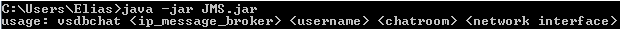
\includegraphics[width=6in]{pic/help.png}
  \item[Falsches Interface angegeben] \hfill \\
    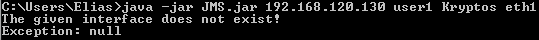
\includegraphics[width=6in]{pic/wrongiface.png}
  \item[Falscher Hostname] \hfill \\
    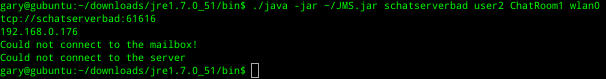
\includegraphics[width=6in]{pic/badhost.png}
  \end{description}
\end{center}

\newpage

\bibliography{protokoll}{}
\bibliographystyle{plain}

\end{document}
